\documentclass[10pt,titlepage]{article}

\usepackage{graphicx}
\usepackage{graphics}
\usepackage{epsfig}
\usepackage{amsmath}
\usepackage{amssymb}
\usepackage{amsthm}
\usepackage{booktabs}
\usepackage{stmaryrd}
\usepackage{url}
\usepackage{longtable}
\usepackage[figuresright]{rotating}
\usepackage[utf8]{inputenc}
\usepackage{svg}
\usepackage[T1]{fontenc}
\usepackage[polish]{babel}
\usepackage{geometry}
\usepackage{pslatex}
\usepackage{ulem}
\usepackage{lipsum}
\usepackage{listings}
\usepackage{url}
\usepackage{color}
\usepackage[ruled,vlined,linesnumbered]{algorithm2e}
\usepackage{listingsutf8}


\definecolor{szary}{gray}{0.6}% jasnoszary

\setlength{\textwidth}{400pt}
% JS listing type
\definecolor{lightgray}{rgb}{.9,.9,.9}
\definecolor{darkgray}{rgb}{.4,.4,.4}
\definecolor{purple}{rgb}{0.65, 0.12, 0.82}

\lstdefinelanguage{JavaScript}{
  keywords={typeof, new, true, false, catch, function, return, null, catch, switch, var, if, in, while, do, else, case, break},
  keywordstyle=\color{blue}\bfseries,
  ndkeywords={class, export, boolean, throw, implements, import, this},
  ndkeywordstyle=\color{darkgray}\bfseries,
  identifierstyle=\color{black},
  sensitive=false,
  comment=[l]{//},
  morecomment=[s]{/*}{*/},
  commentstyle=\color{purple}\ttfamily,
  stringstyle=\color{red}\ttfamily,
  morestring=[b]',
  morestring=[b]"
}
% end JS listing
\lstset{numbers=left,
      numberstyle=\tiny,
      basicstyle=\scriptsize\ttfamily,
      breaklines=true,
      captionpos=b,
      tabsize=2,
      extendedchars=\true,
      inputencoding=utf8}

%listing codes definitions
\lstdefinestyle{sharpc}{language=[Sharp]C}
\newcommand{\includecode}[2][c]{\lstinputlisting[caption=#2, escapechar=, style=custom#1]{#2}}

\selectlanguage{polish}

\newcommand{\RR}{\mathbb{R}}
\newcommand{\NN}{\mathbb{N}}
\newcommand{\QQ}{\mathbb{Q}}
\newcommand{\ZZ}{\mathbb{Z}}
\newcommand{\TAB}{\hspace{0.50cm}}
\newcommand{\IFF}{\leftrightarrow}
\newcommand{\IMP}{\rightarrow}

\newtheorem{theorem}{Twierdzenie}[section]
\newtheorem{lemma}{Lemat}[section]
\newtheorem{example}{Przykład}[section]
\newtheorem{corollary}{Wniosek}[section]
\newtheorem{definition}{Definicja}[section]

\makeindex

\begin{document}
\nocite{*}
\pagestyle{empty}

\begin{titlepage}
\vspace*{\fill}
\begin{center}
\begin{picture}(300,510)
  \put( 10,520){\makebox(0,0)[l]{\large \bf \textsc{Wydział Podstawowych Problemów Techniki}}}
  \put( 10,500){\makebox(0,0)[l]{\large \bf \textsc{Politechniki Wrocławskiej}}}
  \put( 70,280){\makebox(0,0)[l]{\Huge  \bf \textsc{Zarządzanie wydatkami}}}
  \put( 70,240){\makebox(0,0)[l]{\Huge  \bf \textsc{w gospodarstwie domowym}}}
  \put(100,210){\makebox(0,0)[l]{\large     \textsc{Artur Ptaszek}}}

  \put(170, 80){\makebox(0,0)[l]{\large  {Praca inżynierska napisana}}}
  \put(170, 60){\makebox(0,0)[l]{\large  {pod kierunkiem}}}
  \put(170, 40){\makebox(0,0)[l]{\large  {dr Wojciecha Macyny}}}

  \put(100,-80){\makebox(0,0)[bl]{\large \bf \textsc{Wrocław 2014}}}
\end{picture}
\end{center}
\vspace*{\fill}
\end{titlepage}

\tableofcontents

\newpage

\pagestyle{headings}

\section*{Wstęp}
Praca swoim zakresem obejmuje stworzenie aplikacji do zarządzania wydatkami w gospodarstwie \linebreak i wyświetlanie wielu statystyk z nimi związanymi. Ma ona na celu ułatwienie w takim zarządzaniu poprzez wyświetlanie licznych wykresów. Użytkownikiem docelowym jest każdy zarabiający/studiujący chcący organizować swoje wydatki. Celem pracy zaprojektowanie i oprogramowanie aplikacji o następujących założeniach funkcjonalnych:
\begin{itemize}
  \item Dostosowanie interfejsu do szerokiego wachlarzu urządzeń (telefony komórkowe, tablety, komputery)
  \item SPA (Single Page Application) czyli aplikacja działająca bez odświeżenia strony
  \item Prosty i intuicyjny interfejs
  \item Logowanie i rejestracja użytkowników
  \item Wprowadzanie i edycja przychodów i wydatków
  \item Tagowanie przychodów i wydatków
  \item Filtrowanie wydatków (po tagach i po czasie)
  \item Możliwość sprawdzenia czy można sobie pozwolić na jakiś większy wydatek w przyszłych miesiącach (Symulacja)
  \item Możliwość tworzenia wyzwań na tagi czyt. ustawienie sobie jakiegoś limitu na konkretną jednostkę czasu
  \item Możliwość tworzenia wykresów z podsumowaniami wydatków dla tagów
  \item Stworzenie predefiniowanych wykresów
    \begin{itemize}
      \item Wykres kołowy ukazujący wykorzystanie tagowania w wydatkach
      \item Wykres liniowy ukazujący stosunek przychodów do wydatków w ostatnim roku
      \item Wykres liniowy ukazujący bilans przychodów do wydatków w ostatnim roku
      \item Wykres liniowy ukazujący stosunek przychodów do wydatków w ostatnim miesiącu
    \end{itemize}
\end{itemize}
Istnieje wiele aplikacji o podobnej funkcjonalności, które zazwyczaj są połączone z kontem bankowym:
\begin{itemize}
  \item mBank - posiada interfejs do zarządzania wydatkami
  \item ING Bank - posiada interfejs do zarządzania wydatkami
  \item MoneyWiz - Personal Finance
  \item Money (with sync)
  \item Bills
  \item iFinance
\end{itemize}
lecz aplikacja będzie w formie strony internetowej, przez co będzie dostępna na wszystkie platformy. Także idea Responsive Web Design będzie zwiększała zasięg platformowy. Aplikacja mBanku i ING jest bardzo mało intuicyjna przez co można trafić do klientów tych aplikacji. Praca składa się z n rozdziałów ...

\section{Zagadnienia}
W pracy zostały wykorzystane liczne technologie, wzorce i zagadnienia, które poniżej zostaną omówione.
\subsection{SPA - Single Page Application}
Jest to koncepcja, która mówi, że strona powinna być załadowana raz, a każde przejście na kolejną stronę ma być wykonywane asynchronicznie. Wszystkie zmiany strony są pokazywane przez modyfikację drzewa DOM w dokumencie HTML. Uzasadnieniem tego typu stron są rosnące doświadczenia użytkownika przy korzystaniu z aplikacji (User Experience), a także zminimalizowanie transferu danych między przeglądarką a serwerem, przez co czas odpowiedzi serwera jest zdecydowanie szybszy i użytkownik szybciej zobaczy efekt. Koncepcja wiele czerpie z najnowszych technologii jakimi są HTML5, CSS3, JavaScript, AJAX.
\subsection{MVC}
Złożony wzorzec architektoniczny służący do organizowania struktury aplikacji posiadających interfejsy graficzne. Wykorzystuje on 3 proste wzorce jakimi są Strategia, Obserwator, Kompozyt.\linebreak
MVC zakłada podzielenie aplikacji na poniżej wymienione częście składowe:
\begin{itemize}
  \item Model - dane wymagane do utworzenia Widoku
  \item Widok - opisuje jak przedstawić część modelu użytkownikowi
  \item Kontroler - agreguje dane z wielu modeli i przygotowuje je aby przekazać do widoku
\end{itemize}
\subsection{Logowanie tokenowe}
Logowanie to działa na podobnej zasadzie jak logowanie przy pomocy ciasteczek, lecz znosi pewne ograniczenia jakie wcześniej wspomniany i najpopularniejszy w dzisiejszych czasach system identyfikacji sesji posiadał.Użytkownik, który chce się zalogować wpisuje swój login i hasło, na których podstawie jest generowany token (identyfikator sesji), który z kolei podajemy przy każdym wymagającym autentykacji żądaniu do serwera (poprzez dodanie w nagłówku żądania HTTP pola \verb|Authetication: Bearer <token>|). Token jest wydawany jedynie na określony czas i służy do autentykacji tylko dla jednego użytkownika. Jedną z zalet tego logowania jest to, że możemy \linebreak w aplikacjach SPA zalogować się bez odświeżenia strony i dodatkowo aplikacje klienckie możemy ``hostować'' na innej domenie. Nowoczesne strony wykorzystują już tego typu logowanie, idealnym przykładem jest protokół OAuth 2, który wykorzystują liczne strony:
\begin{itemize}
  \item Facebook
  \item Google+
  \item Twitter
\end{itemize}
\begin{figure}[htbp]
  \centering
  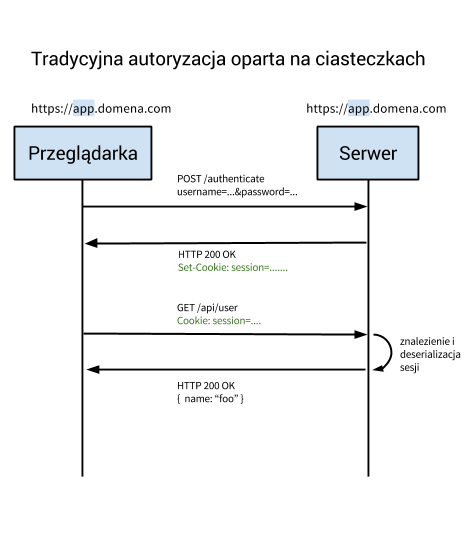
\includegraphics[scale=0.5]{images/tokenAuth1.png}
  \caption{Diagram przepływu dla logowania tradycyjnego}
\end{figure}
\begin{figure}[htbp]
  \centering
  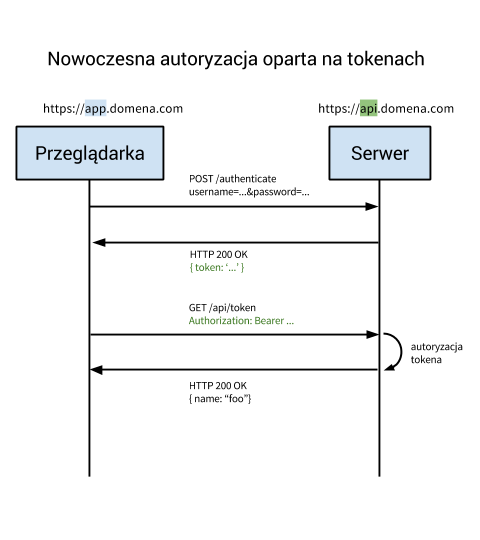
\includegraphics[scale=0.5]{images/tokenAuth2.png}
  \caption{Diagram przepływu dla logowania tokenowego}
\end{figure}
\section{Technologie}
Aplikacja została podzielona na 2 części logiczne, którymi są:
\begin{itemize}
  \item Serwer
  \item Klient
\end{itemize}
Każda z nich używa innych technologii, ponieważ działają w różnych środowiskach np. klient pracuje jedynie w przeglądarce.
\subsection{Serwer}
Została napisana w języku C\# wykorzystując ASP.NET MVC 5 i ASP.NET Web Api 2. Statyczne pliki są udostępniane przy pomocy MVC, a reszta serwera została udostępniona w formie Web Service'u.\\ Silnik bazy danych, który został wykorzystany jest to Microsoft SQL Server 2012 w wersji Express LocalDB. Cała baza danych została zaprojektowana i wygenerowana przy pomocy Entity Framework 6, który także wspomaga wykonywanie zapytań do bazy danych. Zapytania w tej bibliotece nie wykonuje się bezpośrednio przy pomocy języka strukturalnego SQL, lecz pisząc kod i operując na encjach te zapytania są generowane w locie. Wielką zaletą tego typu rozwiązania jest możliwość przeniesienia aplikacji na inny silnik bazy danych bez zmiany jakiegokolwiek fragmentu kodu. Jedyną rzeczą, którą trzeba będzie wykonać to zmienić parametry połączenia. Jest to typowe rozwiązanie mapowania obiektowo-relacyjnego w skrócie ORM.
\subsection{Klient}
Klient został zaimplementowany przy pomocy biblioteki AngularJS. Jest to narzędzie napisane w JavaScript, które umożliwa tworzenie aplikacji za pomocą wzorca projektowego MVC, a także ułatwia tworzenie według koncepcji Single Page Application.\\ Interfejsu graficzny wykorzystuje bibliotekę Bootstrap, która nie tylko ładnie i schludnie wygląda, lecz przy zastosowaniu pewnych reguł zapewnia nam kompatybilność z innymi urządzeniami tj. telefony komórkowe, tablety, czytniki itd. Tego typu zgodność jest nazywana Responsive Web Desing i jest coraz częściej stosowana w internecie.\\ Wykresy są generowane przy pomocy HighCharts.js, który sprawia, że wykresy są proste w generowaniu.\\ Aplikacja została napisana modułowo i każdy takich modułów da się przetestować testami jednostkowymi, a wszystko dzięki narzuconemu schematowi przez AngularJS.
\section{Baza danych}
Jak wyżej zostało napisane baza danych to Microsoft SQL Server 2012 Express LocalDB
Poniżej projekt bazy danych.
\subsection{Diagramy przedstawiające zależności między tabelami}
\begin{figure}[htbp]
  \centering
  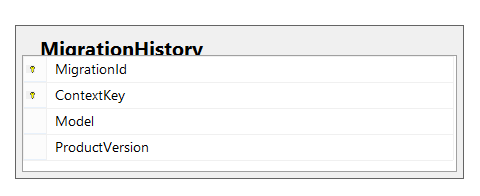
\includegraphics[scale=0.5]{images/db2.png}
  \caption{Tabela migracyjna}
\end{figure}
\begin{figure}[htbp]
  \centering
  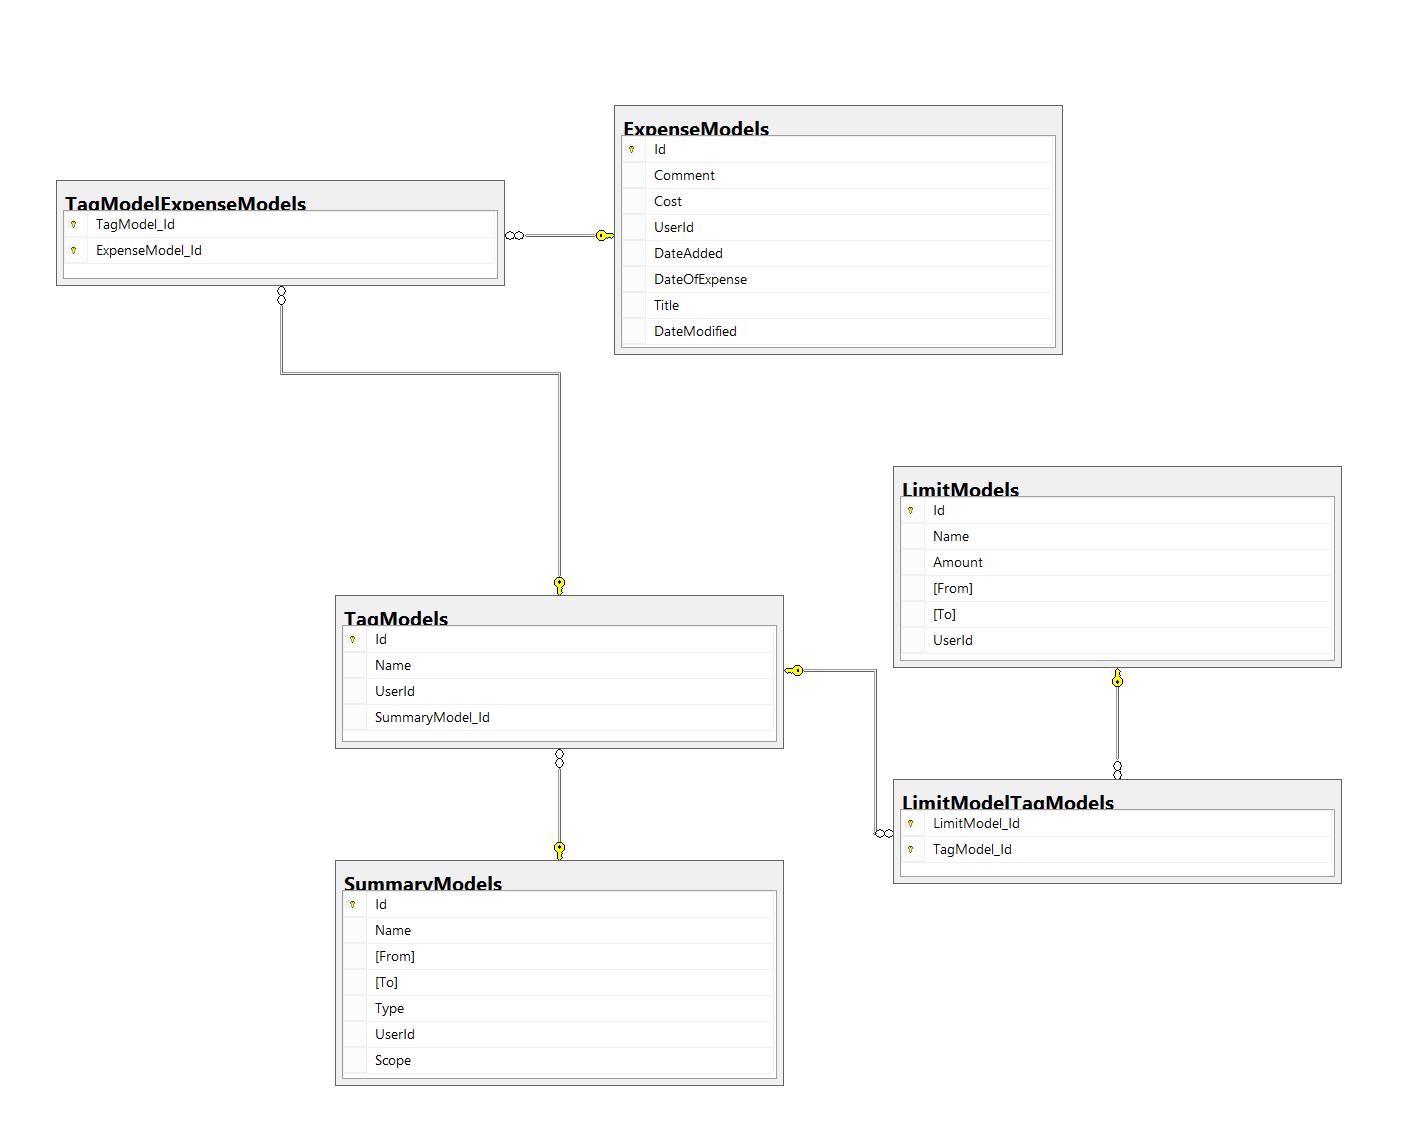
\includegraphics[scale=0.5]{images/db1.png}
  \caption{Tabele aplikacji}
\end{figure}
\begin{figure}[htbp]
  \centering
  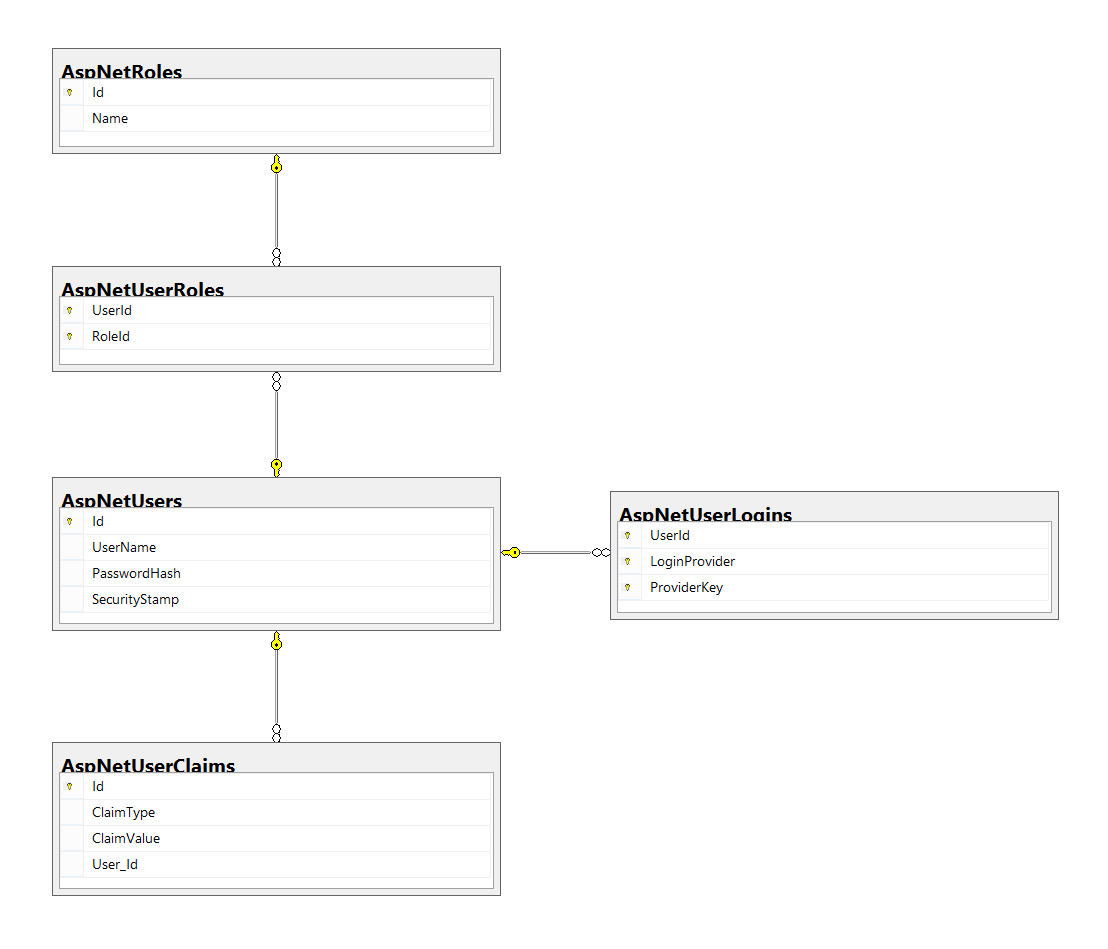
\includegraphics[scale=0.5]{images/db3.png}
  \caption{Tabele autoryzacyjne}
\end{figure}
\subsection{Opis tabel}
\paragraph[short]{ExpenseModels}
Przechowuje wydatki i przychody
\begin{itemize}
  \item Id int IDENTITY (Identyfikator)
  \item Comment nvarchar(max) (Komentarz)
  \item Cost decimal(18,2) (Wartość wydatku/przychodu)
  \item UserId nvarchar(max) (Identyfikator użytkownika)
  \item DateAdded datetime (Data dodania wydatku/przychodu)
  \item DateOfExpense datetime (Data wydatku/przychodu wprowadzona przez użytkownika)
  \item Title nvarchar(max) (Nazwa wydatku)
  \item DateModified datetime (Data modyfikacji wydatku/przychodu)
\end{itemize}
\paragraph[short]{LimitModels}
Przechowuje dane wyzwań
\begin{itemize}
  \item Id int IDENTITY (Identyfikator)
  \item Name nvarchar(max) (Nazwa wyzwania)
  \item Amount decimal(18,2) (Wartość wyzwania)
  \item From datetime (Data, od której zaczyna się wyzwanie)
  \item To datetime (Data, do której trwa wyzwanie)
  \item UserId nvarchar(max) (Identyfikator użytkownika)
\end{itemize}
\paragraph[short]{LimitModelTagModels}
Tabela łącząca tabele wyzwań z tagami
\begin{itemize}
  \item LimitModelId int (Id wyzwania)
  \item TagModelId int (Id tagu)
\end{itemize}
\paragraph[short]{SummaryModels}
Przechowuje dane podsumowań
\begin{itemize}
  \item Id int IDENTITY (Identyfikator)
  \item Name nvarchar(max) (Nazwa podsumowania)
  \item From datetime (Data, od której zaczyna się wyzwanie)
  \item To datetime (Data, do której trwa wyzwanie)
  \item Type int (Typ podsumowania)
  \item Scope int (Zasięg podsumowania np. roczne, miesięczne itd.)
  \item UserId nvarchar(max) (Identyfikator użytkownika)
\end{itemize}
\paragraph[short]{TagModelExpenseModels}
Tabela łącząca tabele wydatków/przychodów z tagami
\begin{itemize}
  \item ExpenseModelId int (Id wydatku/przychodu)
  \item TagModelId int (Id tagu)
\end{itemize}
\paragraph[short]{TagModels}
Tabela przechowująca tagi
\begin{itemize}
  \item Id int IDENTITY (Identyfikator)
  \item Name nvarchar(max) (Nazwa tagu)
  \item UserId nvarchar(max) (Identyfikator użytkownika)
  \item SummaryModelId int (Identyfikator podsumowania)
\end{itemize}
Pozostałe tabele są wykorzystywane przez standardowy mechanizm autentykacji ASP.NET MVC.
\section{Implementacja systemu}
\subsection{Omówienie kodów źródłowych - Serwer}
\lstset{style=sharpc}
\lstinputlisting[caption=Mapowanie ścieżek routingu, label={lst:routeConfig}]{sources/server/routeConfig.cs}
\par Powyższy kod służy do nauczenia serwera IIS interpretowania ścieżek adresu wpisywanych przez użytkownika. Pierwsza linijka metody \verb|RegisterRoutes| jest wymagana przez rozszerzenie Elmah, które służy do monitorowania aplikacji. Mówi ona, że ten typ adresów ma być przez naszą aplikację ignorowany. Adresy, które spełniają ten warunek to np. \verb|http://domena.pl/elmah.axd| lub \verb|http://domena.pl/elmah.axd/1234|. Kolejna użyta metoda jest to napisana na potrzeby aplikacji metoda, która linkuje każdy z adresów pasujących do wyrażeń z pierwszego argumentu metody \verb|MapHtml5Routes| na controller podany w drugim parametrze. Zabieg ten jest wymagany przez router Angular'a, który w aplikacji działa w HTML5Mode i daje na dostęp do adresów URL bez poprzedzania każdej ścieżki znakiem \verb|#|. Kod metody przedstawia Listing \ref{lst:mapHtml5Routes} Podobnym plikiem jest \verb|AngularPlanner/AngularPlanner/App_Start/WebApiConfig.cs|, który ustawia ścieżki routingu lecz dla Web Service'u RESTowego.
\lstinputlisting[caption=Metoda MapHtml5Routes, label={lst:mapHtml5Routes}]{sources/server/mapHtml5Routes.cs}
\par W pliku \verb|AngularPlanner/AngularPlanner/App_Start/BundleConfig.cs| są tworzone paczki plików JavaScript, które na środowisku produkcyjnym są zmiejszone i zoptymalizowane. Zaletą tego rozwiązania są mniejsze transfery danych i szybszy kod po stronie przeglądarki.\par Plik \verb|AngularPlanner/AngularPlanner/App_Start/Startup.Auth.cs| zawiera konfigurację mechanizmu autentykacji tokenowej dla naszej aplikacji. Ponadto istnieje możliwość dodania opcji logowania przez Facebook i Google+.\par Katalog Controllers zawiera klasy kontrollerów są tam przedewszystkim kontrolery Web Api 2, lecz jest tam jeden, który posiada tylko jedną akcję, która z kolei zwraca użytkownikowi widok podany na Listingu \ref{lst:homeIndexView}.
\lstinputlisting[caption=Widok zwracany przez akcję \texttt{Index} kontrolera \texttt{Home}, label={lst:homeIndexView}, language=HTML]{sources/server/homeIndexView.cshtml}
\par Pozostałe kontrollery są do siebie podobne, a kod wybranego z nich można zobaczyć poniżej.
\lstinputlisting[caption=Kontroller ExpensesController, label={lst:expensesController}]{sources/server/expensesController.cs}
\par Klasa kontrollera dziedziczy po klasie abstrakcyjnej ApiController, by mogłabyć rozpoznana przez mechanizm refleksji jako kontroller Web Api 2 i dodatkowo uzyskać dostęp do kilku przydatnych metod charakterystycznych dla tego typu kontrolerów. Trochę wyżej są 2 atrybuty. \verb|Authorize| oznacza, że dostęp do kontrolera mają jedynie zalogowani użytkownicy, a atrybut \verb|ElmahHandleErrorApi| mówi bibliotece Elmah, że ma przechwytywać wyjątki z tego kontrollera. W konstruktorze mamy tworzenie instacji połączenia z bazą danych przy pomocy Entity Framework. W klasie mamy zaimplementowane wszystkie akcje CRUD, czyli Create (metoda \verb|Post|), Read (metody \verb|GetListByDate|, \verb|GetListByTag|, \verb|GetList|, \verb|GetSingle|), Update (metoda \verb|Put|) i Delete (metoda \verb|Delete|). Linia nr 100 przedstawia przykładowe zapytanie do bazy. Odpowiada to zapytaniu w SQLu
\begin{verbatim}
SELECT TOP 1 * FROM dbo.ExpenseModels WHERE UserId = <UserId> AND Id = <Id>
\end{verbatim}
Kolejnym dobrym przykładem zapytania są linie od 78 do 85. Metoda Include robi \verb|LEFT OUTER JOIN| z tabelą \verb|TagsModels|, zaś metoda OrderByDescending dodaje sortowanie po \verb|DateOfExpense| (\verb|ORDER BY DateOfExpense DESC|), \verb|Skip| opuszcza liczbę wpisów podanych w parametrze, a \verb|Take| bierze 20 rekordów. Ważnym elementem tego zapytania jest także \verb|ToListAsync|. Do póki nie użyjemy tej metody zapytanie nie zostanie wykonane, a jedynie przygotowane. Po wykonaniu zapytania (zmaterializowaniu) dane są typu \verb|List|, a wcześniej były \verb|IQueryable|.

\par Pliki w katalogu Models z wyłączeniem \verb|AngularPlannerContext| są to pliki reprezentujące bazę danych. Każda klasa reprezentuje rzeczywistą tabelę w bazie. Dla przykładu została przedstawiony model \verb|Expense| w Listingu \ref{lst:expenseModel}
\lstinputlisting[caption=Model ExpenseModel, label={lst:expenseModel}]{sources/server/expenseModel.cs}
Atrybut \verb|Key| oznacza pole, nad którym się znajduje polem \verb|PRIMARY KEY|. Pole \verb|Tags| jest to tak naprawdę odwołanie do tabeli \verb|TagsModels|. Entity Framework sam stwierdza jakiego typu relacjami mają być połączone tabele w bazie danych (jeden-do-wielu, wiele-do-wielu itd.). Pola \verb|Nullable<DateTime>| oznaczają, że to nie są wymagane i mogą mieć wartość \verb|NULL| w bazie.
\subsection{Omówienie kodów źródłowych - Klient}
\lstset{language=JavaScript}
\par Cały kod aplikacji został zorganizowany według rekomendowanej przez Angulara struktury katalogów ~\cite{angular:structure}.
\par Przy asynchronicznych akcjach jest wykorzystywana okrojona biblioteka \verb|Q.js| ~\cite{lib:q} zaimplementowana w Angularze. Implementuje ona ustandaryzowany system obietnic Promises/A+ ~\cite{doc:promises}
\lstinputlisting[caption=Plik konfiguracyjny systemu budującego Grunt, label={lst:gruntfile}]{sources/client/Gruntfile.js}
\par Kod przestawiony na powyższym listingu jest plikiem konfiguracyjnym dla systemu do automatyzacji pewnych zadań \verb|Grunt|. Można go porównać do \verb|Makefile|, ponieważ jest to narzędzie tego typu, lecz istnieje do niego wiele rozszerzeń, które ułatwiają prace. Powyżej definiujemy 3 zadania: default, test, dev. Każdy z nich można uruchomić za pomocą polecenia \verb|grunt <nazwa_zadania>|. Dev i default nasłuchują katalogi z plikami \verb|*.js|, \verb|*.css|, \verb|*.html|, a następnie robią wstępną kompilację, aby kod napisany był możliwy do pomniejszenia ~\cite{angular:minSafe} i sprawdzany pod względem poprawności składni. Także informowana jest przeglądarka o zmianach, których następstwem jest automatyczne odświeżenie okna przeglądarki. Jest to czynność, która znacznie przyspiesza proces wytwarzania oprogramowania.
\par Plik z Listingu \ref{lst:appJs} jest plikiem startowym aplikacji. Definiuje się tutaj jakie moduły wchodzą w skład aplikacji i konfiguruje środowisko do dalszej pracy. W tym przypadku został włączony \verb|html5Mode| i domyślne przekierowanie na stronę \verb|domena.pl/statistics|. W pliku z Listingu \ref{lst:homeIndexView} jest podłączenie aplikacji do drzewa DOM za pomocą \verb|<body ng-app="app">|.
\lstinputlisting[caption=Plik startowy aplikacji, label={lst:appJs}]{sources/client/app.js}
Mechanizm autentykacji po stronie klienta został napisany na podstawie książki ~\cite{angular:bookMastering}. Jest on podzielony na trzy moduły. Pierwszy z nich przedstwiony na Listingu \ref{lst:authInterceptor} pośredniczy przy żadaniach \linebreak i odpowiedziach dodając \verb|Token| w nagłówkach żądania, jeśli jest on zapisany w \verb|localStorage| przeglądarki. Jeśli \verb|Token| wygaśnie lub jest nieprawidłowy serwer poinformuje klienta statusem kodu \verb|401 - Unauthorized| ~\cite{http:statuscodes}
\lstinputlisting[caption=Moduł pośredniczący przy żądaniach i odpowiedziach HTTP, label={lst:authInterceptor}]{sources/client/authInterceptor.js}
Kolejnym jest przedstawiony na Listingu \ref{lst:authJs} moduł udostępniający najważniejsze metody do autentykacji i sprawdzenia zalogowania użytkownika.
\lstinputlisting[caption=Moduł wystawiający interfejs do autentykacji, label={lst:authJs}]{sources/client/auth.js}
\par Udostępnia on metody \verb|login|, \verb|logout|, \verb|register|, \verb|isAuthenticated|. W przypadku \verb|login| serwer jest odpytywany czy użytkownik z takimi danymi logowania istnieje w bazie danych, jeżeli tak jest to w odpowiedzi dostajemy \verb|Token| autoryzacyjny, który zostaje zapisany w pamięci przeglądarki.
\par Ostatnim z modułów odpowiedzialnych za logowanie jest przedstwiony poniżej. Sprawdza jedynie on w trakcie ładowania widoków, czy mogą być pokazane użytkownikowi. Adresy końcowe dla autentykacji zostały zaczęrpnięte z tutoriala ~\cite{server:tokenLogin}.
\lstinputlisting[caption=Moduł sprawdzający czy dany widok jest dostępny dla anonimowego użytkownika, label={lst:authCheckerJs}]{sources/client/authChecker.js}
\par Do wymiany danych używany jest mechanizm \verb|$resource| ~\cite{angular:$resource}. Przykład implementacji przedstawiony został na Listingu \ref{lst:summaryJs}. Udostępnia on łatwy interfejs do komunikacji z serwerem.
\lstinputlisting[caption=Tags Resouce, label={lst:summaryJs}]{sources/client/summaries.js}
\par Zastosowanie w/w mechanizmu jest podane w Listingu \ref{lst:tagsPickerJs}. Poprzez \verb|Tags.query(callback)| odpytujemy się serwer o listę wszystkich tagów na serwerze. Poprzez utworzenie nowej instancji tworzymy nowy tag, a wywołując na nim metodę \verb|.$save(callback)| zapisujemy go na serwerze.
\lstinputlisting[caption=Dyrektywa <tags-picker />, label={lst:tagsPickerJs}]{sources/client/tagsPicker.js}
\par Warto także wspomnieć, że Listing \ref{lst:tagsPickerJs} tworzy nowy element HTMLa, który jest nazwany \verb|<tags-picker />|. Definicja takiego elementu jest zawarta w liniach od 94 do 104. Parametr \verb|scope| nakazuje utworzyć obiekt podgląd, który jest obiektem dla tego elementu. Danymi źródłowymi są atrybuty dostarczone do elementu. Wartość \verb|'='| nakazuje zachować \verb|2-way data binding| ~\cite{angular:databinding} między widokiem, a kontrolerem dla tej właściwości. \verb|controller| wskazuje, który kontroler ma być wykorzystany. Jest on zaimplementowany wyżej. Parametr \verb|resrict| determinuje jakiego typu ma być dyrektywa ~\cite{angular:restrict}. Więcej o konfiguracjach można przeczytać ~\cite{angular:$compile}.
\par Metody i właściwości są udostępnianie widokowi przy pomocy \verb|$scope|. W kontrolerze jest kilka przykładów: \verb|$scope.delete = function(){}|, \verb|$scope.tags = []|. Także dla właściwości w \verb|$scope| udostępniony został mechanizm obserwowania zmian w tej własciwości. Jest to klasyczne zastosowanie wzorca \verb|Obserwator|. Istnieje też system wiadomości, w którym możemy nasłuchiwać na konkretną wiadomość (\verb|$scope.$on('tagsPicker:push')|) i je wysyłać w górę drzewa podglądów (\verb|$scope.$emit('tagsPicker:push')|) lub w dół (\verb|$scope.$emit('tagsPicker:push')|).
\lstinputlisting[caption=Widok dla dyrektywy <tags-picker />, label={lst:tagsPickerHTML}, language={HTML}]{sources/client/tagsPicker.html}
\par W widoku podpięte są metody na akcje. Dla przykładu można podać \verb|ng-click="delete($index)"| na kliknięcie w element wywołuje tą metodę z kontrolera. Atrybut \verb|ng-repeat="tag in tagsList"| nakazuje powielić element, do którego jest podpięty tyle razy ile jest elementów w tablicy \verb|tagsList|.
\lstinputlisting[caption=Przykładowy kod podstrony, label={lst:expensesCtrl}]{sources/client/expensesController.js}
\par Na samej górze mamy definicje adresów, które prowadzą do podstrony. Każdy z nich ma podany widok i kontroler, przez które będzie obsługiwany adres. W właściwości są zależności, które są wymagane do przejścia na podstronę np. \verb|currentUser: authCheckerProvider.require| jest odpowiedzialny za autoryzację. Jeżeli, któraś z tych zależności nie zostanie spełniona to przejście nie zostanie wykonane, a sam \verb|$routeProvider| wyśle komunikat \verb|$routeChangeError| ~\cite{angular:$routeChangeError}. Poniżej mamy definicję samego kontrolera.
\section{Instalacja i wdrożenie}
Aby wdrożyć aplikację musimy potrzebujemy następujących składników:
\begin{itemize}
  \item Microsoft Windows 2012 Server/7/8 lub wyższe
  \item .NET Framework 4.5
  \item Microsoft SQL Server 2012 lub wyższe
\end{itemize}

\par {\color{red} Tutaj piękna instrukcja instalacji. (Jak zainstaluje nową wirtualną maszynę)}
%%%%%%%%%%%%%%%%%%%%%%%%%%%%%%%%%%%%%%%%%%%%%%%%%%%%%%%%%%%%%%%%%%%%%%%%%%%%%%
%%%%%%%%%%%%%%%%%%%%%%%%%%%%%%% BIBLIOGRAFIA %%%%%%%%%%%%%%%%%%%%%%%%%%%%%%%%%
%%%%%%%%%%%%%%%%%%%%%%%%%%%%%%%%%%%%%%%%%%%%%%%%%%%%%%%%%%%%%%%%%%%%%%%%%%%%%%


\bibliography{bibl}
\bibliographystyle{plain}

\end{document}
